\documentclass[12pt]{article}
\usepackage{graphicx}
\usepackage{float}
\usepackage{enumerate}
\usepackage{listings}
\usepackage{pdfpages}

\title{Detection of Unmanned Aerial Vehicles in the RF Spectrum using Machine Learning Techniques}
\author{Robert L. Koehlmoos} % & Richard N. Shmel  
\date{\today}

\begin{document}

\maketitle
\section{Introduction}

Drones have become increasingly common in modern warfare. Previously they allowed the use of air power by governments at relatively lower costs without endangering the lives of service members but were still costly to employ. More recently, the rising utility and lowering price of drones intended for commercial use created opportunity for their use in military settings by asymmetric or near peer threats \cite{TalibanDrones}. Previously unable to afford them, the drones allow threats to gain air reconnaissance and attacks capabilities, with end uses ranging from propaganda to assassination attempts \cite{DroneImagery}.

In what is potentially the first conventional conflict to make heavy use of drones, the 2020 Nagorno-Karabakh was marked by Azerbaijan’s use of modern drones. They proved effective in locating maneuver units and artillery locations which were followed by drone-based attacks which successfully destroyed tanks, artillery, and air defense systems \cite{AzerbaijanDrones}. While to some extent the success of drone tactics can be attributed to the inability of either side to afford modern air defense assets, their effectiveness against the forces traditionally dominant in conventional land warfare, armor, points to drones creating a potential paradigm shift in warfare which will require the creation of new technology and tactics to counter.

One of the major requirements for counter-drone efforts is the detection of drones. Numerous potential sensor sources exist, such as visual, audio, or heat based. One of the most successful methods has been detecting drone presence through the RF signals they use for communication with controllers. This project builds on existing research to detect drones using captures of their RF transmissions.

\section{Literature Review}

Ezuma et al. \cite{DroneDetection} conducted a thorough study into both detecting and classifying drones of varying designs and manufacturers. They separated their research into two major steps, first distinguishing between signal captures containing drones, other sources, or noise and then classifying them. They initially classified captures as containing either a signal source or noise using a Naïve Bayes model, then separated drone sources using signal bandwidth and symbol duration. Finally, 15 candidate features and five machine learning models were tested to determine which achieved the highest accuracy.

Allahham et al. \cite{DroneDataset} present a methodology for the collection of RF captures of drones. They present the experimental setup for controlling the drone to generate the signal and for equipment to generate the capture. They then touch on a labelling and storing the signals as a database for easy retrieval and analysis. While the methodology presented is relatively basic it provides a good baseline of what is possible using available free software, low cost equipment, and open source formats.

\section{Methodology}

Four sources were selected for classification. Two from drones manufactured by different companies, one from a commercial Wi-fi router, and one of Gaussian noise. The manufacturers of the drones will not be included in this paper due to security concerns. Further, as an exploratory effort this paper seeks to establish a viable methodology for future development, so the exact details of the sources are unnecessary to accomplish those goals.

One five second signal capture was created from each source. The signal was captured in a narrow band at 2.4Ghz band at a sampling rate of 1Mhz. This capture was passed through an additional power filter based on a manually selected power level identified based on observations of the power level in the absence of an active signal source. This produced a final capture consisting of five million binary values for each source where each value represents whether the power for a particular microsecond exceeded the threshold.

Both drones were captures while transmitting information to their controllers, the Wi-Fi router was recorded while performing a speed test. The noise was generated using a software Gaussian noise generator.

Features for training models were generated by collecting information on the frames for each capture. Frames are the blocks of communication transmitted by the sources, and it is assumed that when the power threshold is exceeded that indicates a frame is currently being transmitted. Frames were any contiguous block of high power, separated by any sections of low power. The mean frame length and variance were used with the total percent of time spent transmitting frames as the three features to train models. Features were normalized to allow effective use with the neural network model.

Individual observations were created by dividing each capture up into equal sized subsections. Divisions of 10, 25, and 50 subsections per capture were tested. These sections were selected to give a useful number of observations for training, 40 at the minimum, and explore the impact of progressively smaller subsections.

Six models were trained on this data and then tested on out of sample observations to evaluate performance. The six models selected and their hyperparameters are specified in table ~\ref{tab:hyperparameters}. They were selected to represent a range of commonly used machine learning models. Hyperparameters were generally selected by using default's specified in learning algorithms. The notable exception is the use of a linear kernel for the Suppoert Vector Machine (SVM) classifier instead of a radial basis function. The distribution of features shown in the results section demonstrates a linear separation of classes.

\begin{table}[H]
	\caption{Models and Hyperparameters}
	\label{tab:hyperparameters}
	\begin{tabular}{|l|l|}
		\hline
		Model                        & Hyperparameters                                     \\ \hline
		Neural Network               & One hidden layer of size 100, relu activation       \\ \hline
		Decision Tree                & Gini splitting criterion, Minimum 1 sample per leaf \\ \hline
		Random Forest                & 100 trees, Identical to the individual tree         \\ \hline
		Support Vector Machine       & Linear Kernel, tolerance 0.001                      \\ \hline
		Linear Discriminant Analysis & Uses singular value decomposition as a solver       \\ \hline
		Nearest Neighbors            & Uses the 5 nearest neighbors                        \\ \hline
	\end{tabular}
\end{table}

F-score was selected as the performance metric for final model evaluation. The f-score provides a useful metric for multi-class classification problems as it uses both precision and recall in order to prevent the model from creating excessive false positives or negatives without affecting it's measured performance.

\section{Results}

Figures~\ref{fig:10split},~\ref{fig:25split}, and~\ref{fig:50split} show the distribution of features at observation sizes 0.5s, 0.2s, and 0.1s, respectively. These indicate a high degree of potential separability. Using the mean and variance of frame sizes alone appears to be fully separable for all sizes. However, smaller observation windows do lead to larger ranges of values, especially for noise. This is due to the smaller numbers of frames in each observation causing a greater variability. Up time does provide some separability, however mixes portions of each class at the extremes. At the smallest observation size the noise interferes with all classes for all features.

\begin{figure}[H]
	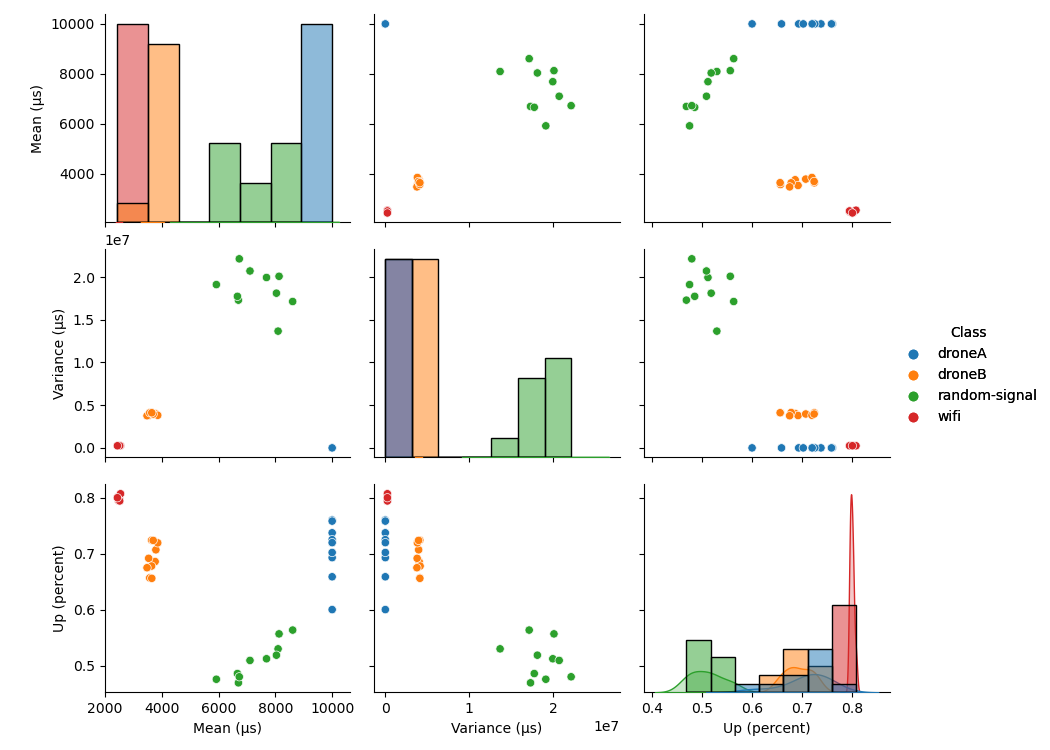
\includegraphics[width=\linewidth]{img/feature_facets_10_splits.png}
	\caption{Distribution of features with 0.5s observations}
	\label{fig:10split}
\end{figure}

\begin{figure}[H]
	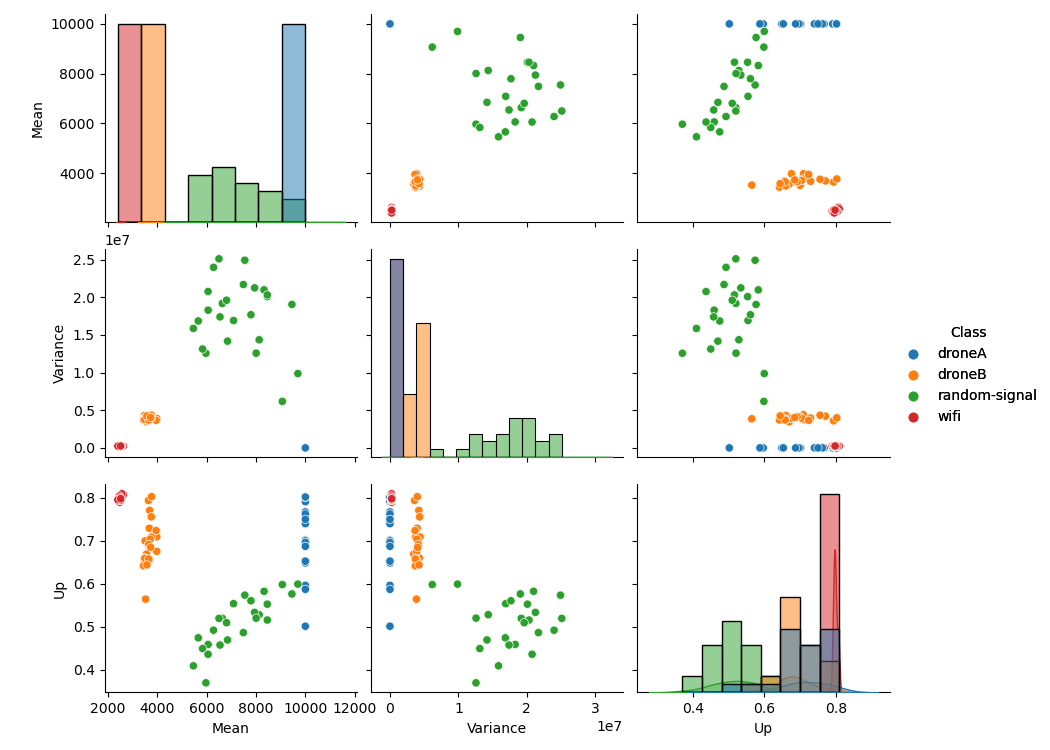
\includegraphics[width=\linewidth]{img/feature_facets_25_splits.png}
	\caption{Distribution of features with 0.2s observations}
	\label{fig:25split}
\end{figure}

\begin{figure}[H]
	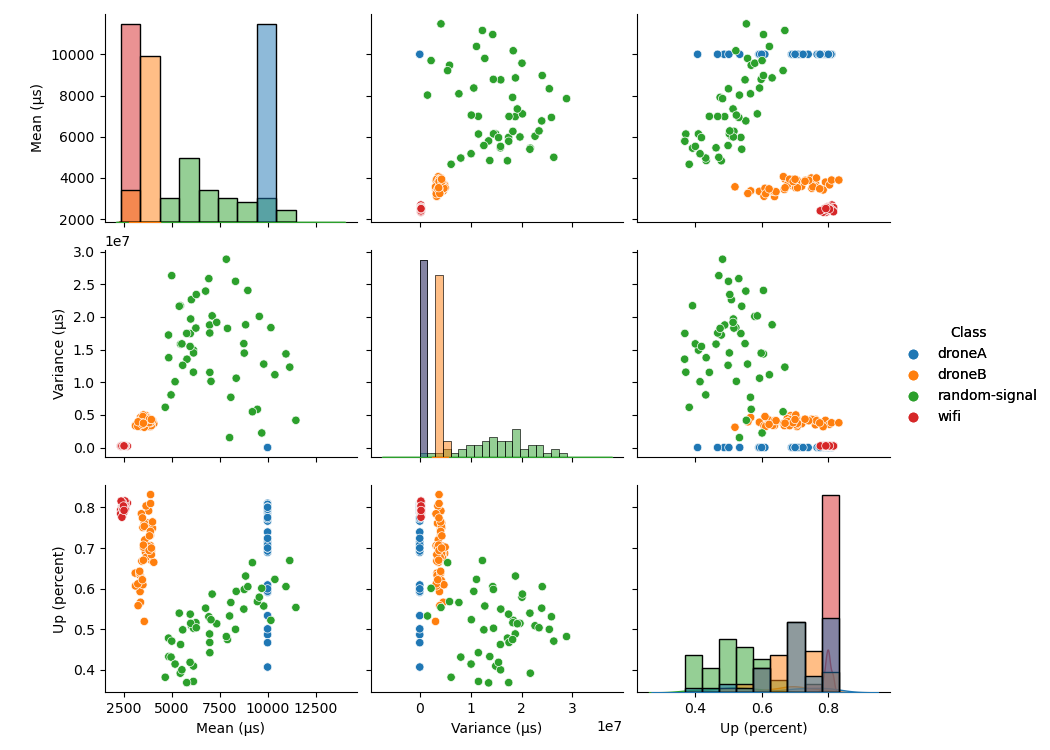
\includegraphics[width=\linewidth]{img/feature_facets_50_splits.png}
	\caption{Distribution of features with 0.1s observations}
	\label{fig:50split}
\end{figure}

% I swear, I could not make this image fit at a reasonable size without breaking the page
Model performance is shown below. All achieved perfect classification at an observation size of 0.5s, all but LDA and the Random Forest models achieved perfect performance at 0.2s, and all showed some errors, but achieved an f-score of over 0.8, for 0.1s samples. No significant differences can be observed between the models. The reduced performance for at smaller samples sizes is a result of the increased overlap between features for different classes observed. Minimal additional analysis is available with the current signal captures.

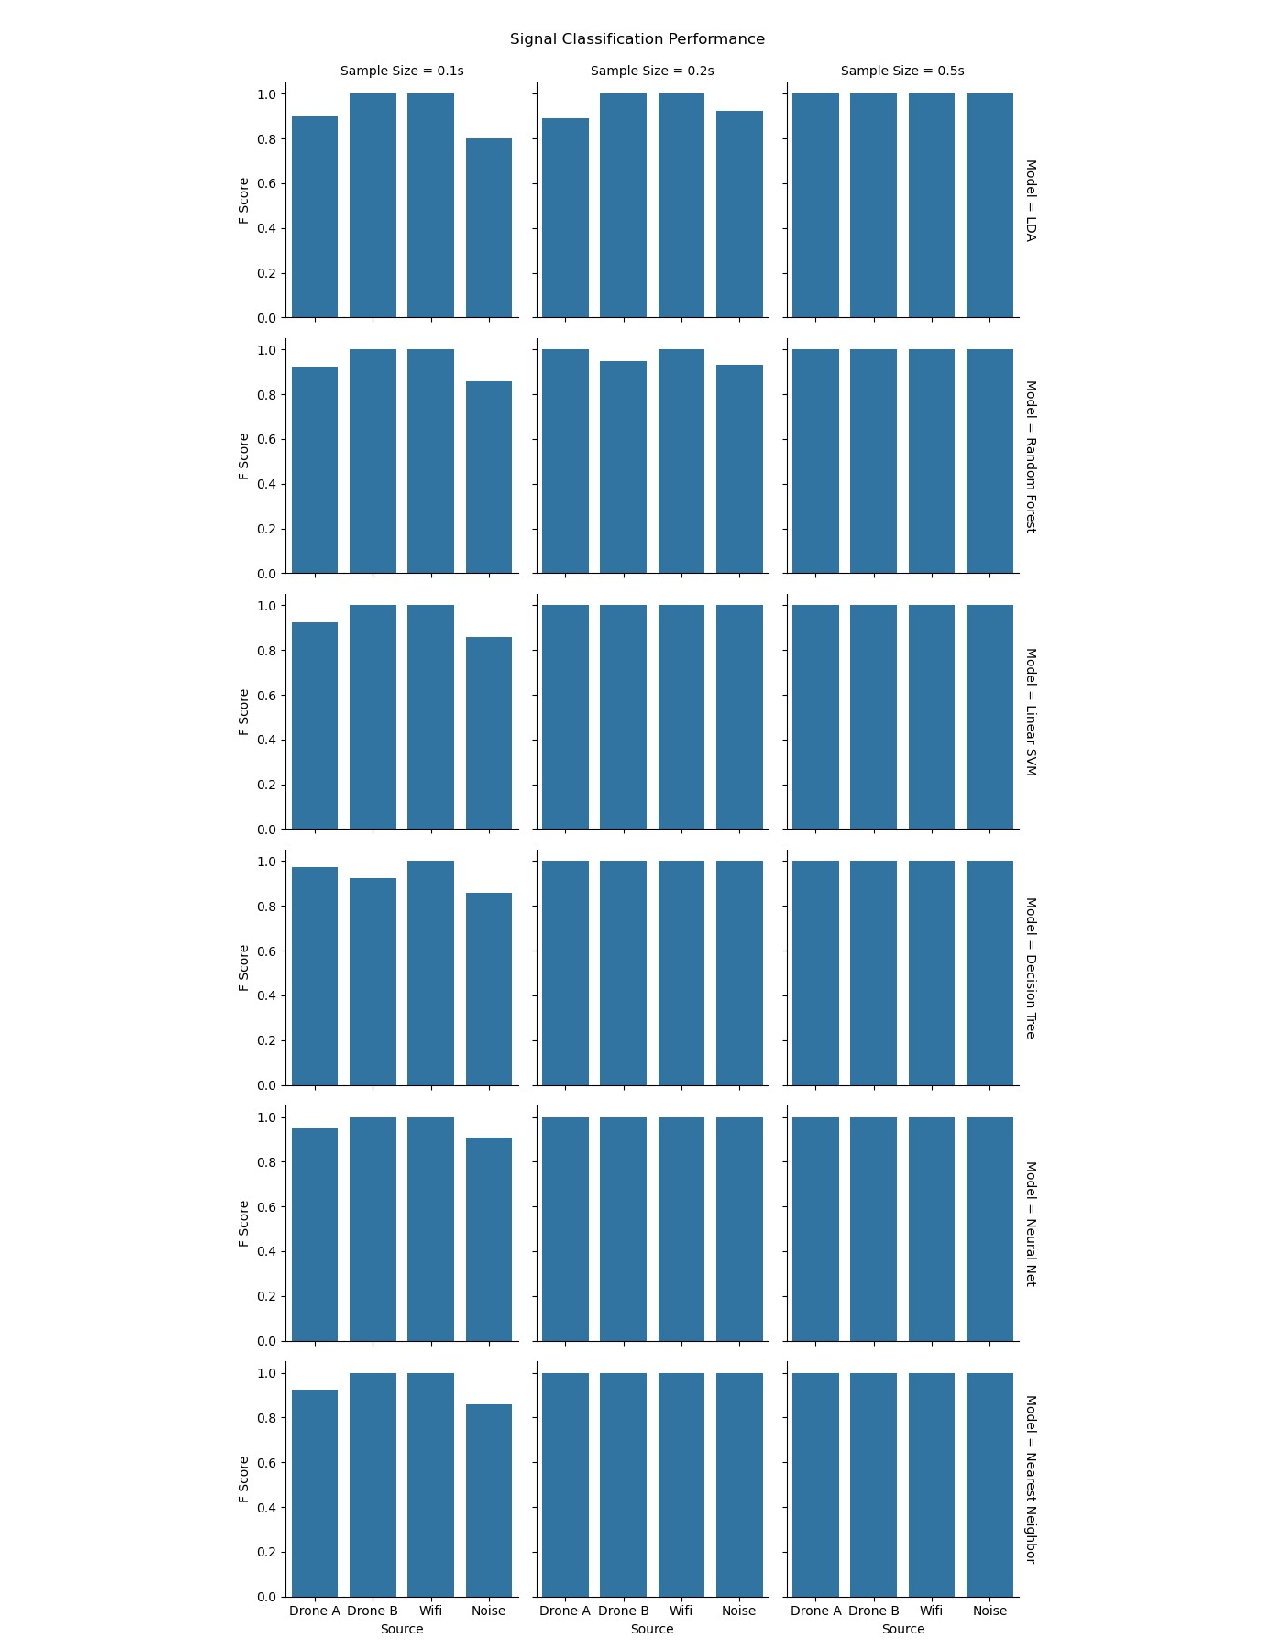
\includepdf{img/performance.pdf}

\section{Conclusion and Future Work}

This paper demonstrates that machine learning models can effectively classify radio signal sources, specifically drones, and differentiate them from noise. All models evaluated showed near perfect performance, additionally all model's require relatively minimal training to achieve those results. This also demonstrates the efficacy of power series as a base for producing training features, which substantially reduced the complexity of equipment required to produce the series compared to capturing the full signal waveform including IQ data, as was used in previous work. With additional exploration these techniques could provide fast and reliable methods of general signal detection and classification in a range of environments.

As this paper seeks only to explore whether the techniques described could prove effective there remain clear avenues of work for future work to improve their efficacy. A wider range of signal captures for training and testing of models needs to be provided. A short five second capture may not be sufficient for measuring the full range of potential features each source will generate. Signal captures should be taken for longer periods of time and across a range of activities. They can also be taken with other sources running in range of the capture device to test the ability of models to classify the primary signal source. As a greater range of captures become available the size of observations can be optimized to find a preferred balance between performance and run time. Finally, model hyper parameters can continue to be tuned as additional captures increase the model complexity required.

\begin{thebibliography}{5}
	\bibitem{DroneDataset} 
	Allahham, Mhd Saria, Mohammad F. Al-Sa'd, Abdulla Al-Ali, Amr Mohamed, Tamer Khattab, and Aiman Erbad. 
	\textit{DroneRF Dataset: A Dataset of Drones for RF-Based Detection, Classification and Identification}. 
	 Data in Brief 26 (2019): 104313. https://doi.org/10.1016/j.dib.2019.104313.
	 
	\bibitem{DroneImagery} 
	Archambault, Emil, and Yannick Veilleux-Lepage. 
	\textit{Drone Imagery in Islamic State Propaganda: Flying like a State.}.
	International Affairs, July 1, 2020. https://doi.org/10.1093/ia/iiaa014
	
	\bibitem{AzerbaijanDrones} 
	Dixon, Robyn.
	\textit{Azerbaijan’s Drones Owned the Battlefield in Nagorno-Karabakh — and Showed Future of Warfare}.
	The Washington Post, November 11, 2020.
	
	\bibitem{DroneDetection}
	Ezuma, Martins, Fatih Erden, Chethan Kumar Anjinappa, Ozgur Ozdemir, and Ismail Guvenc. 
	\textit{Detection and Classification of UAVs Using RF Fingerprints in the Presence of Wi-Fi and Bluetooth Interference}.
	IEEE Open Journal of the Communications Society 1 (2020): 60–76. https://doi.org/10.1109/ojcoms.2019.2955889
	
	\bibitem{TalibanDrones}
	Rahim, Najim, and Thomas Gibbons-neff. 
	\textit{Deadly Taliban Attack Probably Used Drone, a Worrisome Shift}.
	The New York Times. The New York Times, November 1, 2020. https://www.nytimes.com/2020/11/01/world/asia/taliban-drone-afghanistan.html
\end{thebibliography}

\end{document}